\documentclass[12pt,titlepage]{article}

\usepackage[top=1.75in,left=1.5in,right=1.5in,bottom=1.25in,verbose]{geometry}%footskip=.25in,
\usepackage{graphicx}
\usepackage{rotating}
\usepackage{amssymb,amsmath}\allowdisplaybreaks[4]
\usepackage{multirow}
\usepackage{fancyhdr}
\usepackage{overpic}
\usepackage{epsfig}
\usepackage{setspace}
\usepackage{makeidx}
\usepackage{epsfig}
\usepackage{paralist}
\usepackage{appendix}
\usepackage{changebar}
\usepackage[round]{natbib}

\newcounter{funnum}
\newcommand{\fthefunnum}{F\thefunnum}
\newcommand{\fref}[1]{F\ref{#1}}

\newcounter{nfnum}
\newcommand{\nthenfnum}{N\thenfnum}
\newcommand{\nref}[1]{N\ref{#1}}

\newcounter{goalnum}
\newcommand{\gthegoalnum}{G\thegoalnum}
\newcommand{\gref}[1]{G\ref{#1}}

\newcounter{assnum}
\newcommand{\atheassnum}{A\theassnum}
\newcommand{\aref}[1]{A\ref{#1}}

\newcounter{tmnum}
\newcommand{\tmthetmnum}{TM\thetmnum}
\newcommand{\tmref}[1]{TM\ref{#1}}

\newcounter{ddnum}
\newcommand{\dtheddnum}{D\theddnum}
\newcommand{\dref}[1]{D\ref{#1}}

\newcounter{acnum}
\newcommand{\actheacnum}{AC\theacnum}
\newcommand{\acref}[1]{AC\ref{#1}}

\newcounter{ucnum}
\newcommand{\uctheucnum}{UC\theucnum}
\newcommand{\uref}[1]{UC\ref{#1}}

\newcounter{mnum}
\newcommand{\mthemnum}{M\themnum}
\newcommand{\mref}[1]{M\ref{#1}}

\newcounter{qfnum}
\newcommand{\qftheqfnum}{QF\theqfnum}
\newcommand{\qfref}[1]{QF\ref{#1}}

\newcounter{casenum}
\newcommand{\cthecasenum}{TC\thecasenum}
\newcommand{\cref}[1]{TC\ref{#1}}

\newcommand{\mi}[1]{#1\index{#1}}
%\makeindex

\addtocounter{secnumdepth}{3}

\newcommand{\colAwidth}{0.36\textwidth}
\newcommand{\colBwidth}{0.45\textwidth}
\newcommand{\firstCol}{0.17\textwidth}
\newcommand{\secondCol}{0.7\textwidth}
\newcommand{\colOne}{0.1\textwidth}
\newcommand{\colTwo}{0.15\textwidth}

\DeclareGraphicsRule{.jpg}{eps}{}{}

\pagestyle{fancy}
\renewcommand{\headrulewidth}{0pt}
\renewcommand{\footrulewidth}{0pt}
\fancyhf{} \fancyfoot[C]{\thepage} \fancyhead[C]{\itshape Wen Yu -- McMaster University -- Computing and Software}

\setlength{\parindent}{0.5in}

\newcommand{\HRule}{\rule{\linewidth}{0.5mm}}
%\doublespacing

\author{Wen Yu}

\begin{document}

\begin{titlepage}

% Fonts for the title page
\newcommand{\texttl}{\textsf} %font for the title (Emil's version is \textsf)
\newcommand{\textau}{\textsf} %font for the authors, date, etc. (Emils version is \textsc)

\begin{center}
 
\HRule \\[0.4cm]
{ \huge \bfseries \texttl{Summary of Validation Testing for a Parallel Mesh Generation Toolbox}}\\[0.4cm]
 
\HRule \\[2cm]

\textau{\LARGE Wen Yu}\\[2cm]
 
\textau{\LARGE {September 2008}}
 
\vfill
 
% Bottom of the page
%\includegraphics[width=0.27\textwidth]{logo.pdf}
\hfill
\textau{\LARGE
\raisebox{2pt}{\begin{tabular}[b]{r}
\raisebox{8pt}{Computing and Software} \\
McMaster University \end{tabular}}
}
\end{center}

\end{titlepage}

\tableofcontents

%to get cross-references correct
\refstepcounter{funnum} \label{RefiningMesh}
\refstepcounter{funnum} \label{CoarseningMesh}
\refstepcounter{funnum} \label{RefiningOrCoarsening}
\refstepcounter{funnum} \label{MeshType}
\refstepcounter{funnum} \label{ElmShape}
\refstepcounter{funnum} \label{DomainDimension}
\refstepcounter{funnum} \label{Conformal}
\refstepcounter{funnum} \label{InputDefinition}
\refstepcounter{funnum} \label{RCInstruction}
\refstepcounter{funnum} \label{OutputStorage}
\refstepcounter{funnum} \label{VertexUniqueID}
\refstepcounter{funnum} \label{ElmUniqueID}
\refstepcounter{funnum} \label{ElmTopology}
\refstepcounter{funnum} \label{OutElmOrder}
\refstepcounter{funnum} \label{OutVertexOrder}
\refstepcounter{funnum} \label{Help}
\refstepcounter{nfnum} \label{Performance}
\refstepcounter{nfnum} \label{Precision}
\refstepcounter{nfnum} \label{Exception}
\refstepcounter{nfnum} \label{Portability}
\refstepcounter{nfnum} \label{LookAndFeel}
\refstepcounter{nfnum} \label{Usability}
\refstepcounter{nfnum} \label{Maintainability}

\refstepcounter{mnum} \label{mMemory}
\refstepcounter{mnum} \label{mFileRW}
\refstepcounter{mnum} \label{mKeyboard}
\refstepcounter{mnum} \label{mScreen}
\refstepcounter{mnum} \label{mInput}
\refstepcounter{mnum} \label{mOutput}
\refstepcounter{mnum} \label{mService}
\refstepcounter{mnum} \label{mVertex}
\refstepcounter{mnum} \label{mEdge}
\refstepcounter{mnum} \label{mCell}
\refstepcounter{mnum} \label{mMesh}
\refstepcounter{mnum} \label{mRefining}
\refstepcounter{mnum} \label{mCoarsening}

\newpage

\section{Introduction \label{AtestSecIntro}}
This section gives an overview of the Testing Summary for a Parallel Mesh Generation Toolbox (PMGT). First, the purpose of the document is provided. Second, the scope of the testing is identified. Third, the organization of the document is summarized.

\subsection{Purpose of the Document}
This document specifies validation tests for a PMGT. The results of the tests and analysis are also provided. The intended audience is testers who are going to test the system and developers who are going to maintain the software. Note that test document is dynamic in the sense that it should be updated when the development of the system proceeds. 

\subsection{Scope of the Testing }
In general, the purpose of testing is to help produce quality software. Due to limits on the time available for testing, the scope of the testing of PMGT is restricted to test the most important test factors. Like other scientific computing software, correctness and efficiency are considered to be the two most important test factors for PMGT. For efficiency testing, the focus is on execution time rather than on storage. 

\subsection{Organization of the Document}
Section \ref{AtestSecIntro} (this section) is an introduction to the report. Section \ref{AtestSecTest} shows what is going to be tested and the coverage of the testing, with respect to the software requirements and the software design. Section \ref{AtestSecResult} gives the result of the testing and the analysis. 

\section{Testing PMGT \label{AtestSecTest}}
Test cases are listed in Section \ref{AtestSecTestcases}. The detailed information for these test cases can be found in Section \ref{AtestSecResult}. The traceability matrix in Section \ref{AmatrixR} shows the association between test cases and the functional and nonfunctional requirements that are specified in the Software Requirements Specification (SRS) document. Similarly, a traceability matrix for test cases and the leaf modules as introduced in the Module Guide (MG) as shown in Section \ref{AmatrixM}. Tracking these relations is useful for developing and maintaining the software.

\subsection{Test Cases \label{AtestSecTestcases}}
The correctness validation test is designed for verifying the functional requirements RefiningMesh (\fref{RefiningMesh}), CoarseningMesh (\fref{CoarseningMesh}), ElmShape (\fref{ElmShape}), and Conformal (\fref{Conformal}). Other requirements for correctness are trivial and are satisfied obviously. For example, since the vertices are stored in an array, the OutVertexOrder (\fref{OutVertexOrder}) requirement is met by outputting the vertices in the order as the order of them in the array. The tests are against above requirements are automated. The automated validation tests requirements (ACVTRs) are listed in Section \ref{ACVTRs}. Since the output mesh also can also be displayed on screen, it can be checked manually. The visual correctness validation tests requirements (VCVTRs) are listed in Section \ref{VCVTRs}. The test cases are in Section \ref{TCs}.
\subsubsection{Automated Correctness Validation Tests Requirements \label{ACVTRs}} 
A list of ACVTRs follows. All test cases should pass these tests. Some test cases relate to data definitions defined in the SRS. In these cases the related data definition defined is shown as D$x$, where $x$ is the number of the associated data definition given in the SRS. 
\begin{itemize}
\item The area of each element is greater than zero (referring to \textbf{D5}). %hard coded reference
\item The boundary of the mesh is closed. (referring to \textbf{D15}). %hard coded reference
\item The mesh is conformal (referring to \textbf{D16}). %hard coded reference
\item The intersection of any two elements is empty (referring to \textbf{D17}). %hard coded reference
\item The input mesh and output mesh {\em CoveringUp} each other (referring to \textbf{D19}). %hard coded reference
\item The length of each edge is greater than zero. (This is required by the definition of a mesh, which is defined in the SRS.)
\item The vertices of each element are listed in a counterclockwise order. (The counterclockwise order of the vertices for each element is not necessary for implementing PMGT. However, it is adopted by most meshing and FEA software. PMGT uses this convention.) 
\item The output mesh conforms to the Euler Equation. (This requirement is not documented in the SRS. However, any mesh should implicitly satisfy the equation $nc+nv-ne=1$, where $nc$ is the number of cells, $nv$ is the number of vertices, and $ne$ is the number of edges.)
\end{itemize}
\subsubsection{Visual Correctness Validation Tests Requirements\label{VCVTRs}}
The output meshes should also be visually checked to ensure that the following VCVTRs are met.
\begin{itemize}
\item No vertex is outside of the input domain.
\item No vertex is inside of a cell.
\item No dangling points or edges are present.
\item All cells are connected.
\item The mesh is conformal.
\end{itemize}
Some of the VCVTRs overlap with the ACVTRs. This redundancy provides increased confidence in case one testing method fails to catch an error. 
\subsubsection{Test Cases\label{TCs}}
The test cases developed involve testing meshes against the above requirements. In each test case, except the last one, the input mesh is refined and then coarsened. Two algorithms for refining are used. One algorithm is called {\em Split}. It splits one cell into three by adding a point in the centroid of the triangle and connecting the added point to the three original vertices. The other algorithm is simply call {\em Refine}. It refines the original mesh by longest edge bisection. 

The name of each test case includes three parts. For example, test case $AxxCBN$ means that the test uses $Axx$ algorithm for refining, where $Axx$ equals $Split$ or $Refine$. The letter $C$ indicates that coarsening is performed. If the $C$ is missing, the input mesh is not coarsened. $B$ is the number of refinements before coarsening. If $B$ is S, the mesh is refined once and then coarsen once. If the $B$ is M, the mesh is refined multiple time before coarsening. $N$ is a number. If the $N$ is omitted, it means only one of this kind of test performed. Otherwise the same test procedures is used several times on different input meshes. The reason for using the same procedure is that the topology of the output meshes may differ for different input meshes.
\begin{itemize}
\item Test Case {\em SplitCS} (\refstepcounter{casenum}\cthecasenum \label{ATCscs}): This test case tests the correctness of PMGT. The input mesh is shown in Figure \ref{input1}. The refining and coarsening criterion is that the cells intersected with the vertical line, $x=0.6$, are Split once, then the cells of the new mesh that intersect with the vertical line are coarsened once. When the splitting and coarsening is done, the vertical line is moved to the right one unit ($x=x+1.0$), and another Splitting and coarsening is performed. This procedure is repeated until no cells intersect with the vertical line. 

\item Test Case {\em RefineCS1} (\refstepcounter{casenum}\cthecasenum \label{ATCrcs1}): This test case tests the correctness of PMGT. The input mesh is the same as \cref{ATCscs}, which is shown in Figure \ref{input1}. There is a vertical line at $x = 0.6$. The refining and coarsening criterion is that the cells that intersect with the vertical line are refined once, then the cells of the new mesh that intersect with the vertical line are coarsened once. When the refining and coarsening are done, the vertical line is moved to the right one unit, and another refining and coarsening is performed. This procedure is repeated until no cells intersect with the vertical line. 

\item Test Case {\em RefineCS2} (\refstepcounter{casenum}\cthecasenum \label{ATCrcs2}): This test case tests the correctness of PMGT. The refining and coarsening criterion, vertical line function, and the test procedure are the same as test case \cref{ATCrcs1}. However, the input mesh is different. The input mesh is showed in Figure \ref{input2}. 

\item Test Case {\em RefineCM} (\refstepcounter{casenum}\cthecasenum \label{ATCrcm}): This test case tests the correctness of PMGT. The input mesh is shown in Figure \ref{input3}. There is a vertical line at $x = 0.5$. The refining and coarsening criterion is the size of the cells. The size of the cell is measured by the length of the longest edge of the cell. The cells that intersect with the vertical line are refined until the criterion is met. When the refining is done, the vertical line is moved to the right $0.6$ unit ($x=x+0.6$), and another refinement is performed. After five refinements are done, the cells to be left of the vertical line by up to 2 units are coarsened, until the coarsening criterion is met. The refining and coarsening are stopped when the vertical line moves to a position outside of the domain. 

\item Test Case {\em RefineM} (\refstepcounter{casenum}\cthecasenum \label{ATCrm}): This test case tests the correctness of PMGT. The input mesh is shown in Figure \ref{input4}. There is an arc with radius of 0.7 unit going through the mesh. Cells that intersect with the arc are refined until the required number of refinements has been reached. 

\item Test Case {\em Split} (\refstepcounter{casenum}\cthecasenum \label{ATCss}): This test case tests both the correctness and speed of PMGT. The input mesh is shown in Figure \ref{input5}. This test simply splits all cells of the mesh 4 times. It is done in both the serial version and the parallel version with different number of processors. The execution time of setting the cells to be refined and splitting the cells is measured. 
\end{itemize}

\subsection{Traceability Matrix for SRS \label{AmatrixR}}
In the traceability matrix for software requirements, if a test case tests the functionality of a software requirement, there will be a check mark on the cell for the corresponding test case. In each row of the traceability matrix for software requirements (Table \ref{AtestTMr}), if the requirement in that row defines the correctness or the speed of the software, one or more cells in this row are checked. Otherwise, all cells in the row are empty. Table \ref{AtestTMr} shows that the test cases developed in Section \ref{AtestSecTestcases} assist with validating the correctness and speed of the software. The detailed information for each functional and nonfunctional requirements can be found in the SRS document.
The names of the requirements and their corresponding numbers are listed below for convenience.
\begin{description}
\item[\fref{RefiningMesh}:] RefiningMesh 
\item[\fref{CoarseningMesh}:] CoarseningMesh
\item[\fref{RefiningOrCoarsening}:] RefiningOrCoarsening
\item[\fref{MeshType}:] MeshType
\item[\fref{ElmShape}:] ElmShape
\item[\fref{DomainDimension}:] DomainDimension
\item[\fref{Conformal}:] Conformal
\item[\fref{InputDefinition}:] InputDefinition
\item[\fref{RCInstruction}:] RCInstruction
\item[\fref{OutputStorage}:] OutputStorage
\item[\fref{VertexUniqueID}:] VertexUniqueID
\item[\fref{ElmUniqueID}:] ElmUniqueID
\item[\fref{ElmTopology}:] ElmTopology
\item[\fref{OutElmOrder}:] OutElmOrder
\item[\fref{OutVertexOrder}:] OutVertexOrder
\item[\fref{Help}:] Help
\item[\nref{Performance}:] Performance
\item[\nref{Precision}:] Precision
\item[\nref{Exception}:] Exception
\item[\nref{Portability}:] Portability
\item[\nref{LookAndFeel}:] LookAndFeel
\item[\nref{Usability}:] Usability
\item[\nref{Maintainability}:] Maintainability
\end{description}

\begin{table}[ht]
\centering
\begin{tabular}{|p{0.06\textwidth}|p{0.06\textwidth}|p{0.06\textwidth}|p{0.06\textwidth}|p{0.06\textwidth}|p{0.06\textwidth}|p{0.06\textwidth}|}
\hline
 &\cref{ATCscs} & \cref{ATCrcs1} & \cref{ATCrcs2} & \cref{ATCrcm} & \cref{ATCrm}&\cref{ATCss}\\
\hline\hline
\fref{RefiningMesh}& \checkmark & \checkmark & \checkmark & \checkmark & \checkmark & \checkmark\\\hline%f2
\fref{CoarseningMesh}& \checkmark & \checkmark & \checkmark & \checkmark & &   \\\hline%f3
\fref{RefiningOrCoarsening}& \checkmark & \checkmark & \checkmark & \checkmark & \checkmark & \checkmark \\\hline%f1
\fref{MeshType}& \checkmark & \checkmark & \checkmark & \checkmark & \checkmark&  \\\hline%f4
\fref{ElmShape}& \checkmark & \checkmark & \checkmark &  \checkmark  & \checkmark& \\\hline%f5
\fref{DomainDimension}& \checkmark & \checkmark &  \checkmark  & \checkmark & \checkmark& \\\hline%f6
\fref{Conformal}&  \checkmark &\checkmark & \checkmark & \checkmark & \checkmark& \\\hline%f7
\fref{InputDefinition}& \checkmark & \checkmark & \checkmark & \checkmark & \checkmark & \checkmark \\\hline
\fref{RCInstruction}& \checkmark & \checkmark & \checkmark & \checkmark & \checkmark & \checkmark \\\hline
\fref{OutputStorage}& \checkmark & \checkmark & \checkmark & \checkmark & \checkmark & \\\hline
\fref{VertexUniqueID}& \checkmark & \checkmark & \checkmark & \checkmark & \checkmark & \\\hline
\fref{ElmUniqueID}& \checkmark & \checkmark & \checkmark & \checkmark & \checkmark &  \\\hline
\fref{ElmTopology}& \checkmark & \checkmark & \checkmark & \checkmark & \checkmark &  \\\hline
\fref{OutElmOrder}& \checkmark & \checkmark & \checkmark & \checkmark & \checkmark & \\\hline
\fref{OutVertexOrder}& \checkmark & \checkmark & \checkmark & \checkmark & \checkmark & \\\hline
\fref{Help} & &  &    &  & &  \\\hline
\nref{Performance} &  &  &    &  & & \checkmark \\\hline
\nref{Precision} &  &  &    &  & &  \\\hline
\nref{Exception} & &  &    &  & &  \\\hline
\nref{Portability} & &  &    &  & &  \\\hline
\nref{LookAndFeel} &   &  &    &  & &  \\\hline
\nref{Usability} &   &  &    &  & &  \\\hline
\nref{Maintainability} &  &  &    &  & &  \\\hline
\end{tabular}
\caption{Traceability Matrix: Test Cases and Requirements}
\label{AtestTMr}
\end{table}

\subsection{Traceability Matrix for MG \label{AmatrixM}}
Similar to Section \ref{AmatrixR}, the traceability matrix for modules (Table \ref{AtestTMm}) shows that the test cases validate the modules that are associated with correctness and speed. The names of modules appear in Table \ref{AtestTMm} are listed below. The detailed information for each module can be found in the MG document.
\begin{description}
\item[\mref{mMemory}:] Virtual Memory Module
\item[\mref{mFileRW}:] File Read/Write Module
\item[\mref{mKeyboard}:] Keyboard Input Module
\item[\mref{mScreen}:] Screen Output Module
\item[\mref{mInput}:] Input Format Module
\item[\mref{mOutput}:] Output Format Module
\item[\mref{mService}:] Service Module
\item[\mref{mVertex}:] Vertex Module
\item[\mref{mEdge}:] Edge Module
\item[\mref{mCell}:] Cell Module
\item[\mref{mMesh}:] Mesh Module
\item[\mref{mRefining}:] Refining Module
\item[\mref{mCoarsening}:] Coarsening Module
\end{description}

\begin{table}[ht]
\centering
\begin{tabular}{|p{0.06\textwidth}|p{0.06\textwidth}|p{0.06\textwidth}|p{0.06\textwidth}|p{0.06\textwidth}|p{0.06\textwidth}|p{0.06\textwidth}|}
\hline
 &\cref{ATCscs} & \cref{ATCrcs1} & \cref{ATCrcs2} & \cref{ATCrcm} & \cref{ATCrm}&\cref{ATCss}\\
\hline\hline
\mref{mMemory}& \checkmark & \checkmark & \checkmark & \checkmark & \checkmark & \checkmark \\\hline
\mref{mFileRW}& \checkmark & \checkmark & \checkmark & \checkmark & \checkmark & \checkmark \\\hline
\mref{mKeyboard}& \checkmark & \checkmark & \checkmark & \checkmark & \checkmark & \checkmark \\\hline
\mref{mScreen}& \checkmark & \checkmark & \checkmark & \checkmark & \checkmark & \checkmark \\\hline
\mref{mInput}& \checkmark & \checkmark & \checkmark & \checkmark & \checkmark & \checkmark \\\hline
\mref{mOutput}& \checkmark & \checkmark & \checkmark & \checkmark & \checkmark & \checkmark \\\hline
\mref{mService}& \checkmark & \checkmark & \checkmark & \checkmark & \checkmark &  \\\hline
\mref{mVertex}& \checkmark & \checkmark & \checkmark & \checkmark & \checkmark & \checkmark \\\hline
\mref{mEdge}& \checkmark & \checkmark & \checkmark & \checkmark & \checkmark & \checkmark \\\hline
\mref{mCell}& \checkmark & \checkmark & \checkmark & \checkmark & \checkmark & \checkmark \\\hline
\mref{mMesh}& \checkmark & \checkmark & \checkmark & \checkmark & \checkmark & \checkmark \\\hline
\mref{mRefining}& \checkmark & \checkmark & \checkmark & \checkmark & \checkmark & \checkmark \\\hline
\mref{mCoarsening}& \checkmark & \checkmark & \checkmark & \checkmark &  &  \\\hline
\end{tabular} 
\caption{Traceability Matrix: Test Cases and Modules}
\label{AtestTMm}
\end{table}

\section{Results and Analysis\label{AtestSecResult}}
The results of the test cases defined in Section \ref{TCs} are listed in Section \ref{AtestSectestresult}. The analysis, including charts that compare the execution time of the parallel version to the serial version are provided in Section \ref{AtestSecAnalysis}. 
\subsection {Testing Results \label{AtestSectestresult}}
The following tables list the testing results of each test case. The field {\em Test Case Number} and {\em Test Case Name} list the number and the name of each test case. The {\em Input field} gives the number of the figure that is the input for that test case, or a description of the input mesh. The {\em Expected Output} describes the requirements of the output mesh. The {\em Actual Output} gives the result of the test. The {\em Selected Output Mesh} field should give the output meshes. However, there are too many intermediate mesh to display, and displaying only the final mesh is too simple to illustrate the feature of the test case. Selected intermediate meshes and final mesh are included in the {\em Actual Output} field. The {\em Result} field indicates whether the test is passed or failed.

\vspace{1cm}
\begin{minipage}{\textwidth}
\begin{tabular}{p{\colAwidth}|p{\colBwidth}} 
\hline \hline 
{\bf Test Case Number} & \cref{ATCscs} \\ 
{\bf Test Case Name} & SplitCS\\ 
\hline
Input & Figure \ref{input1}\\
Expected Output & ACVTRs and VCVTRs listed in Section \ref{AtestSecTest} are met\\
Actual Output & Summary of the correctness test:\\
& 15 tests are performed.\\
& 15 tests succeed.\\
& 0 tests fail.\\
Selected Output Mesh &Figure \ref{output11}, \ref{output12}, \ref{output13}\\
Result & Passed\\
\hline \hline
\end{tabular}
\end{minipage}


\vspace{1cm}
\begin{minipage}{\textwidth}
\begin{tabular}{p{\colAwidth}|p{\colBwidth}} 
\hline \hline 
{\bf Test Case Number} & \cref{ATCrcs1} \\ 
{\bf Test Case Name} & RefineCS1\\ 
\hline
Input & Figure \ref{input1}\\
Expected Output & ACVTRs and VCVTRs listed in Section \ref{AtestSecTest} are met\\
Actual Output & Summary of the correctness test:\\
& 15 tests are performed.\\
& 15 tests succeed.\\
& 0 tests fail.\\
Selected Output Mesh & Figure \ref{output21}, \ref{output22}, \ref{output23}\\
Result & Passed\\
\hline \hline
\end{tabular}
\end{minipage}

\vspace{1cm}
\begin{minipage}{\textwidth}
\begin{tabular}{p{\colAwidth}|p{\colBwidth}} 
\hline \hline 
{\bf Test Case Number} & \cref{ATCrcs2} \\ 
{\bf Test Case Name} & RefineCS2\\ 
\hline
Input & Figure \ref{input2}\\
Expected Output & ACVTRs and VCVTRs listed in Section \ref{AtestSecTest} are met\\
Actual Output & Summary of the correctness test:\\
& 15 tests are performed.\\
& 15 tests succeed.\\
& 0 tests fail.\\
Selected Output Mesh & Figure \ref{output31}, \ref{output32}, \ref{output33}\\
Result & Passed\\
\hline \hline
\end{tabular}
\end{minipage}

\vspace{1cm}
\begin{minipage}{\textwidth}
\begin{tabular}{p{\colAwidth}|p{\colBwidth}} 
\hline \hline 
{\bf Test Case Number} & \cref{ATCrcm} \\ 
{\bf Test Case Name} & RefineCM\\ 
\hline
Input & Figure \ref{input3}\\
Expected Output & ACVTRs and VCVTRs listed in Section \ref{AtestSecTest} are met\\
Actual Output & Summary of the correctness test:\\
& 15 tests are performed.\\
& 15 tests succeed.\\
& 0 tests fail.\\
Selected Output Mesh & Figure \ref{output41}, \ref{output42}, \ref{output43}, \ref{output44}\\
Result & Passed\\
\hline \hline
\end{tabular}
\end{minipage}

\vspace{1cm}
\begin{minipage}{\textwidth}
\begin{tabular}{p{\colAwidth}|p{\colBwidth}} 
\hline \hline 
{\bf Test Case Number} & \cref{ATCrm} \\ 
{\bf Test Case Name} & RefineM\\ 
\hline
Input & Figure \ref{input4}\\
Expected Output & ACVTRs and VCVTRs listed in Section \ref{AtestSecTest} are met\\
Actual Output & Summary of the correctness test:\\
& 15 tests are performed.\\
& 15 tests succeed.\\
& 0 tests fail.\\
Selected Output Mesh & Figure \ref{output51}, \ref{output52}, \ref{output53}\\
Result & Passed\\
\hline \hline
\end{tabular}
\end{minipage}

\vspace{1cm}
\begin{minipage}{\textwidth}
\begin{tabular}{p{\colAwidth}|p{\colBwidth}} 
\hline \hline 
{\bf Test Case Number} & \cref{ATCss} \\ 
{\bf Test Case Name} & SplitM\\ 
\hline
Input & Figure \ref{input4}\\
Expected Output & ACVTRs and VCVTRs listed in Section \ref{AtestSecTest} are met\\
& Execution time increases as the number of cells increases. Execution time decreases as the number of processors increases.\\
Actual Output & Execution time as indicated in Figure \ref{output61}\\
Selected Output Mesh & The mesh is too dense to be shown.\\
Result & Passed\\
\hline \hline
\end{tabular}
\end{minipage}

\begin{figure}[ht]
\centering
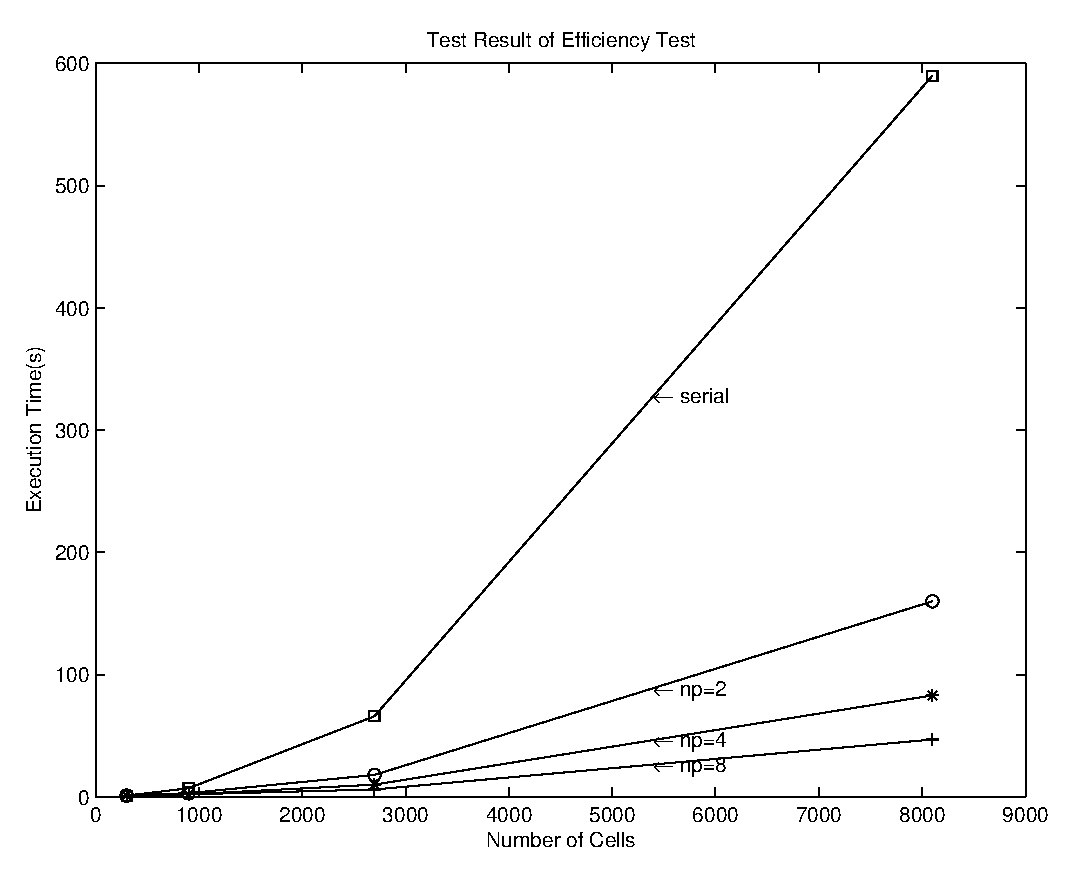
\epsfig{file=output61.eps, width= \textwidth}
\caption{Output of \cref{ATCss}}
\label{output61}
\end{figure}

\subsection {Analysis \label{AtestSecAnalysis}}
All of the test cases conform to the ACVTRs and VCVTRs listed in Section \ref{AtestSecTest}. The test result of \cref{ATCss} show that when the number of cells increased, the execution time increased, and when the number of processors increased, the execution time decreased. That is, this test is passed. Figure \ref{speedup} show the speedup when using different numbers of processors. The speedup is defined as
\[ Speedup(n) = \frac{T_{1}}{T_{n}}
\]
Where $T_{1}$ is the execution time of the serial version, and $T_{n}$ is the execution time of the parallel version with $n$ processors. In general, $Speedup(n) < n$. However, for PMGT, when the number of cells is greater than 2700, $Speedup(n) > n$, which is a super linear speedup. Since the algorithms used for the serial version and the parallel version are the same, the super linear speedup is probably due to the cache effect. That is, when the numbers of processors increases, the size of the accumulated caches from different processors also increases. With the larger accumulated cache size, more, or even all, core data set can fit into the caches and the memory access time reduces dramatically. This may explain the extra speedup in additional to the speedup due to parallel computation.

\begin{figure}
\centering
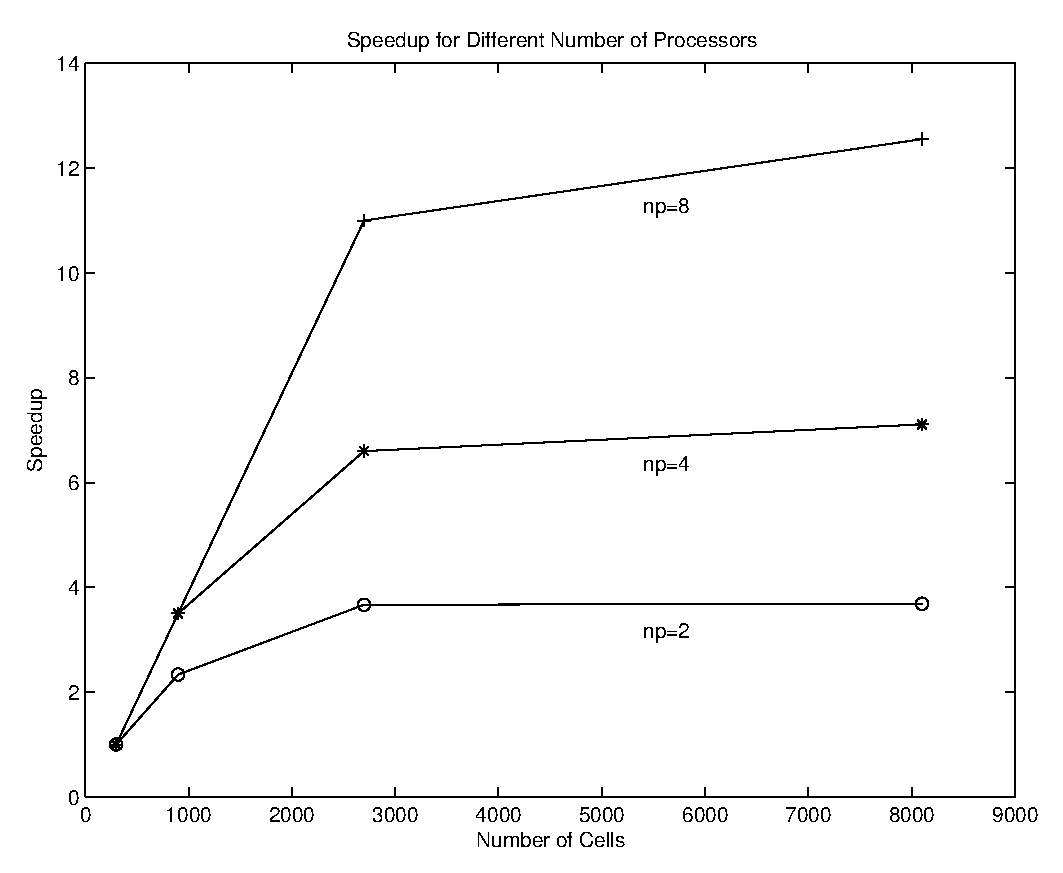
\epsfig{file=speedup.eps, width= \textwidth}
\caption{Speedup for Different Numbers of Processors}
\label{speedup}
\end{figure}


\begin{figure}
\centering
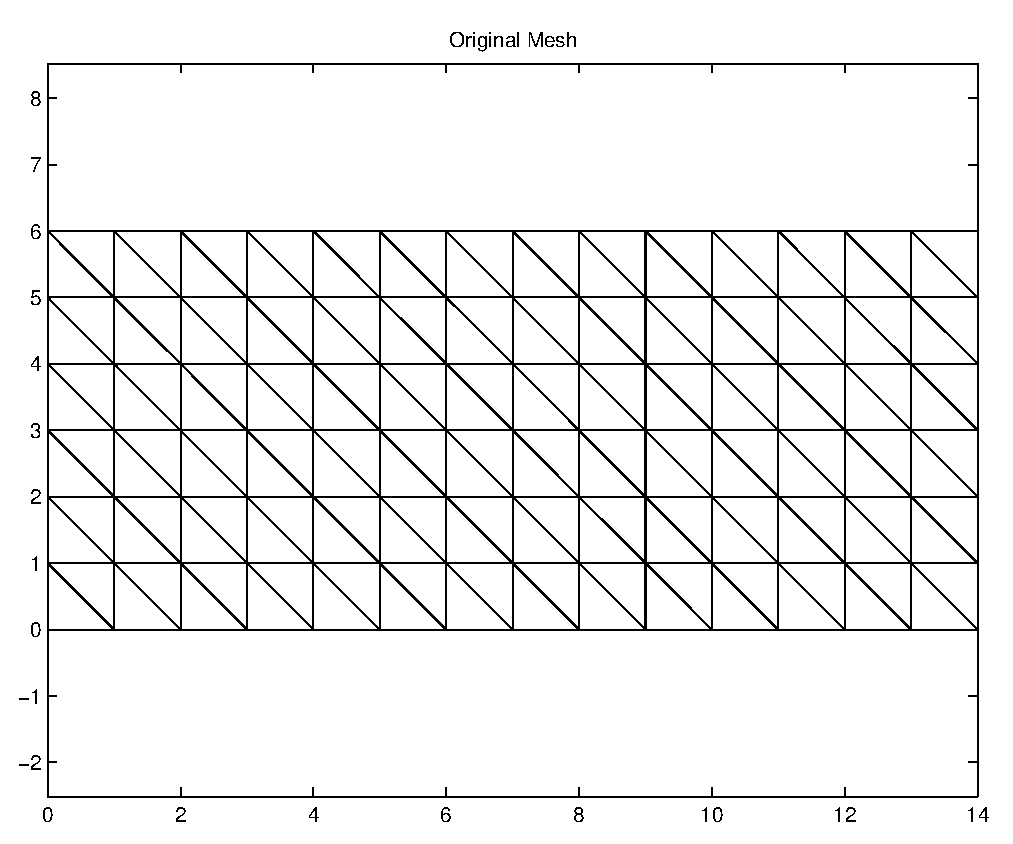
\epsfig{file=input1.eps, width= 0.7\textwidth}
\caption{Input 1}
\label{input1}
\end{figure}

\begin{figure}
\centering
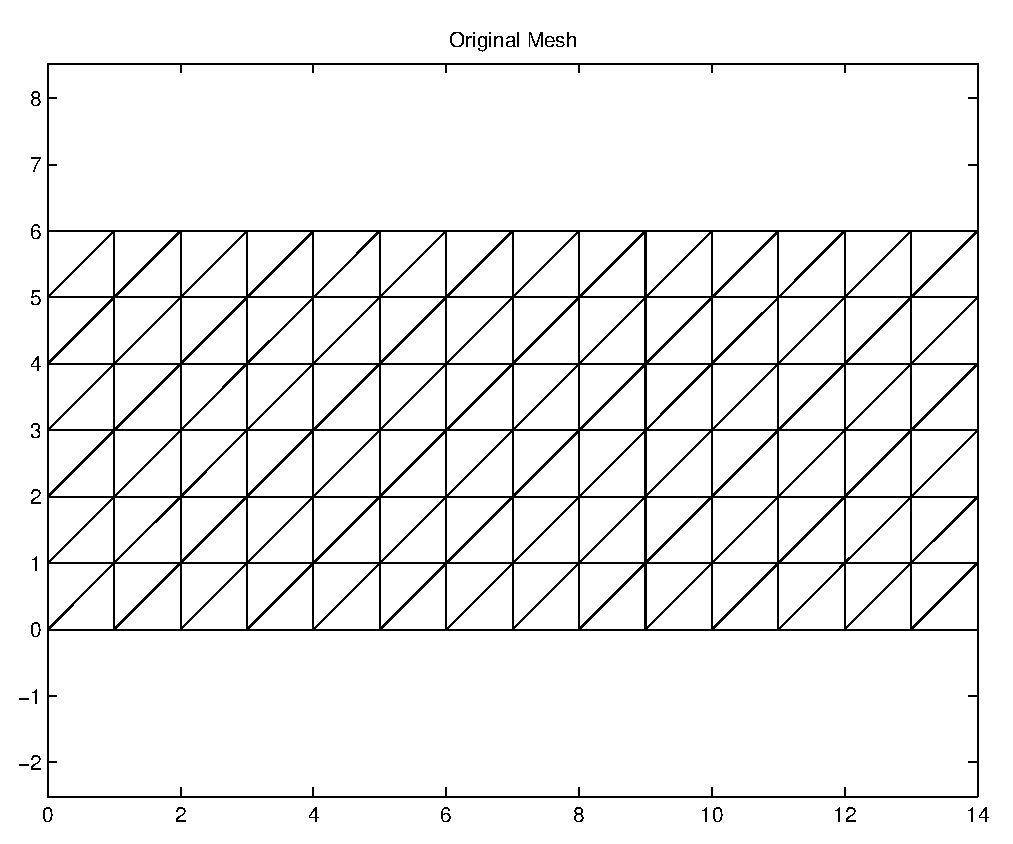
\epsfig{file=input2.eps, width= 0.7\textwidth}
\caption{Input 2}
\label{input2}
\end{figure}

\begin{figure}
\centering
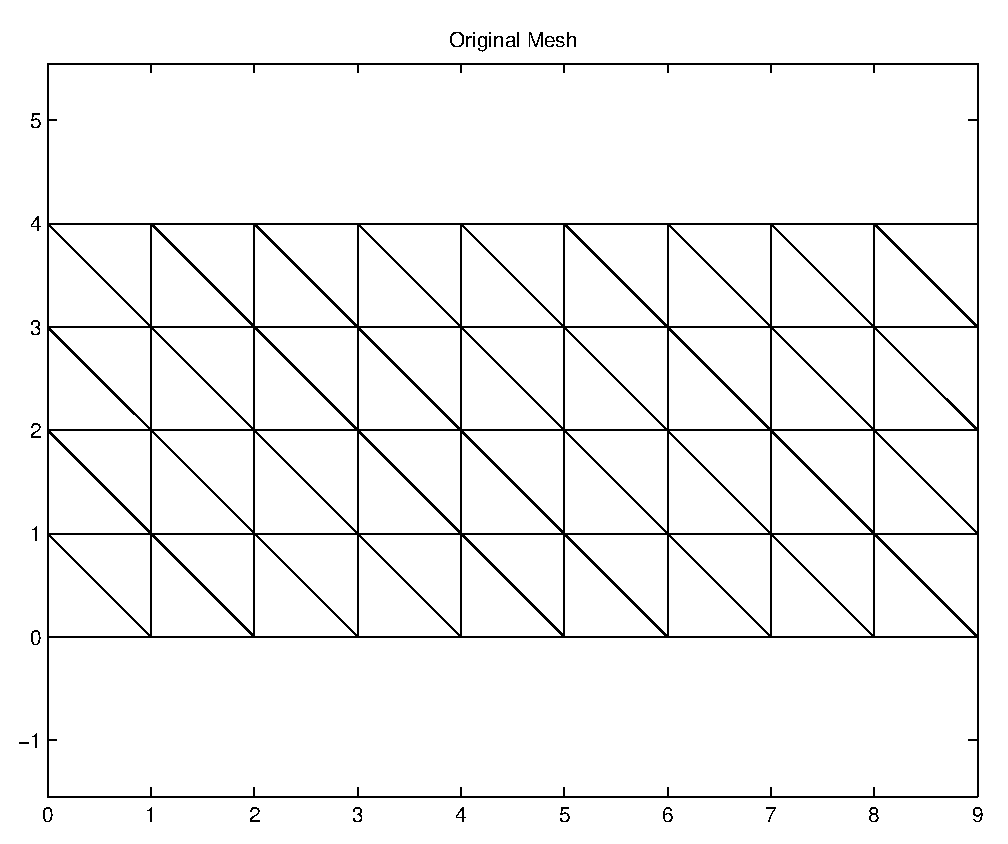
\epsfig{file=input3.eps, width= 0.7\textwidth}
\caption{Input 3}
\label{input3}
\end{figure}

\begin{figure}
\centering
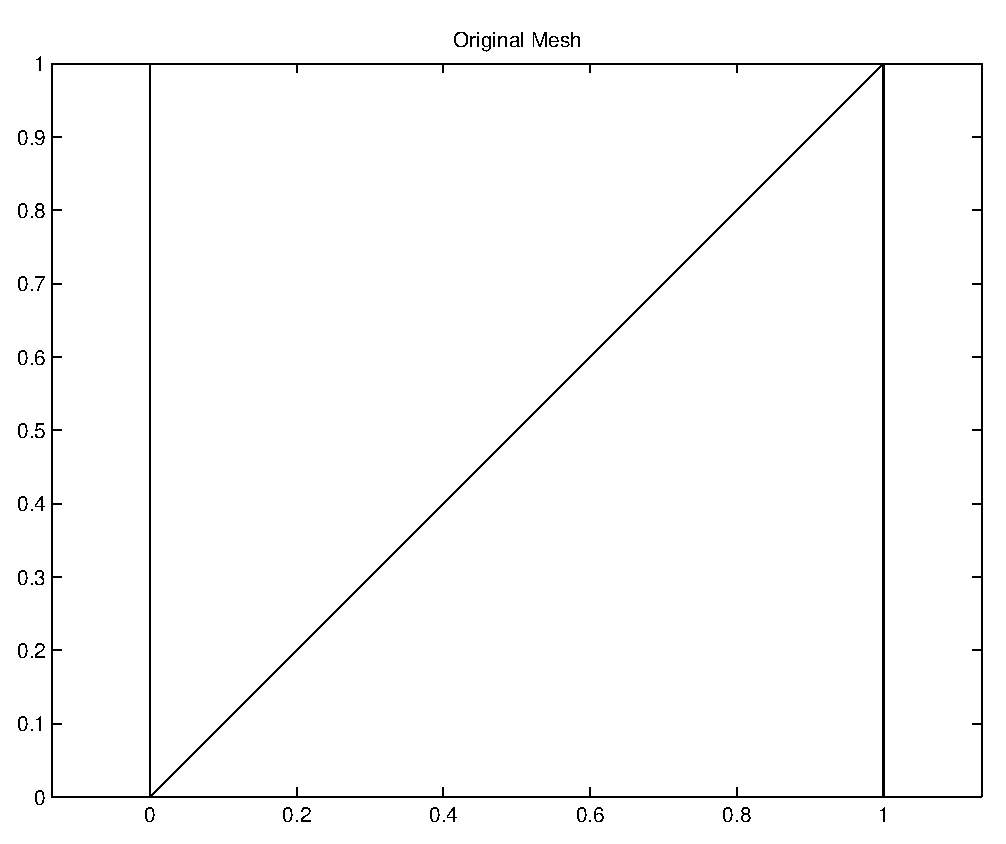
\epsfig{file=input4.eps, width= 0.7\textwidth}
\caption{Input 4}
\label{input4}
\end{figure}

\begin{figure}
\centering
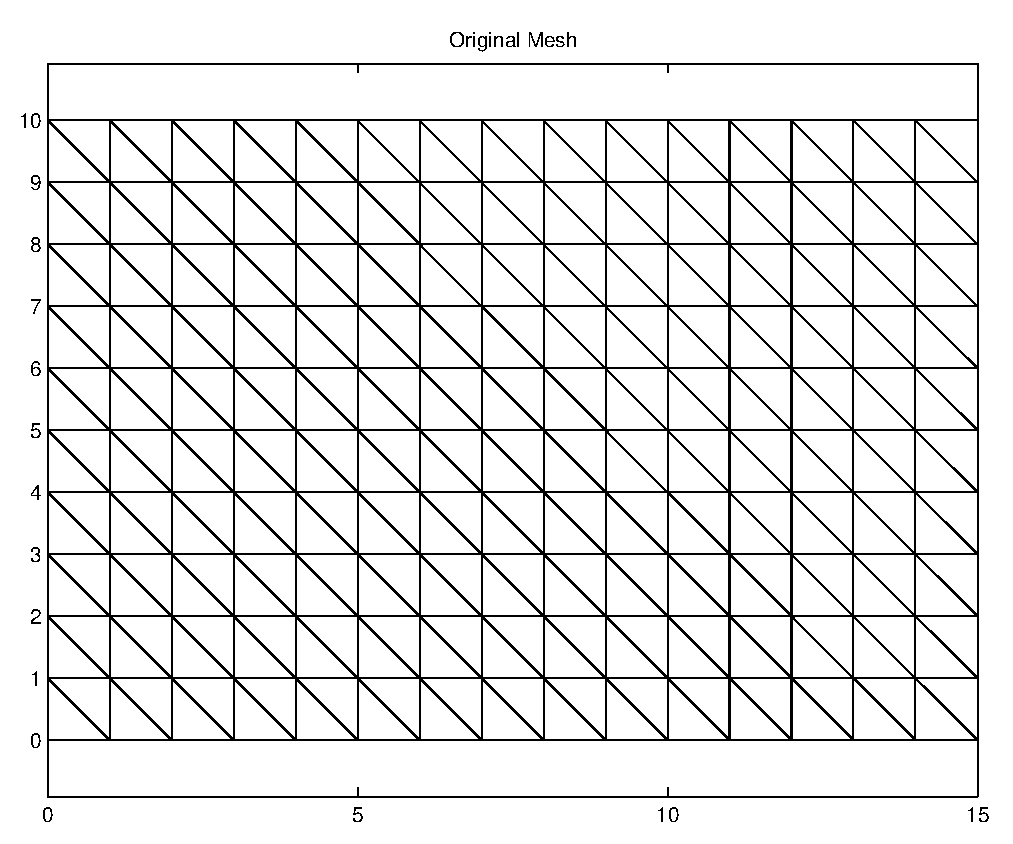
\epsfig{file=input5.eps, width= 0.7\textwidth}
\caption{Input 5}
\label{input5}
\end{figure}

\begin{figure}
\centering
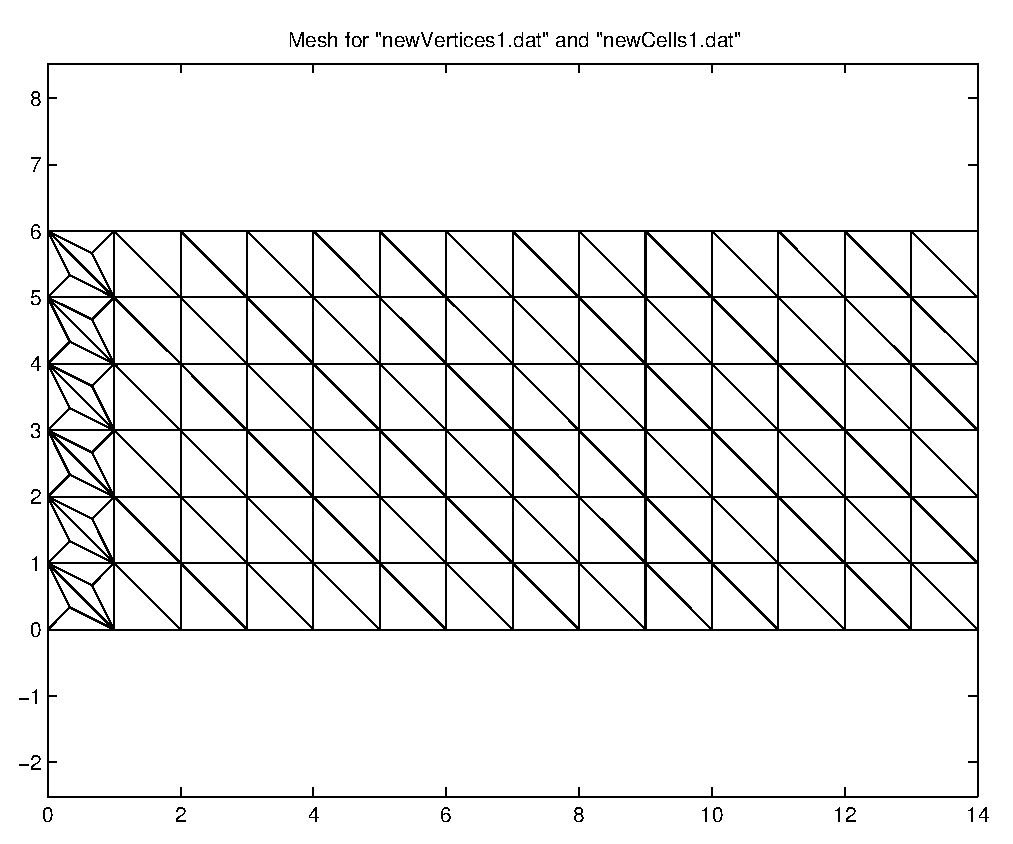
\epsfig{file=output11.eps, width=0.7\textwidth}
\caption{Output 1 of \cref{ATCscs}}
\label{output11}
\end{figure}

\begin{figure}
\centering
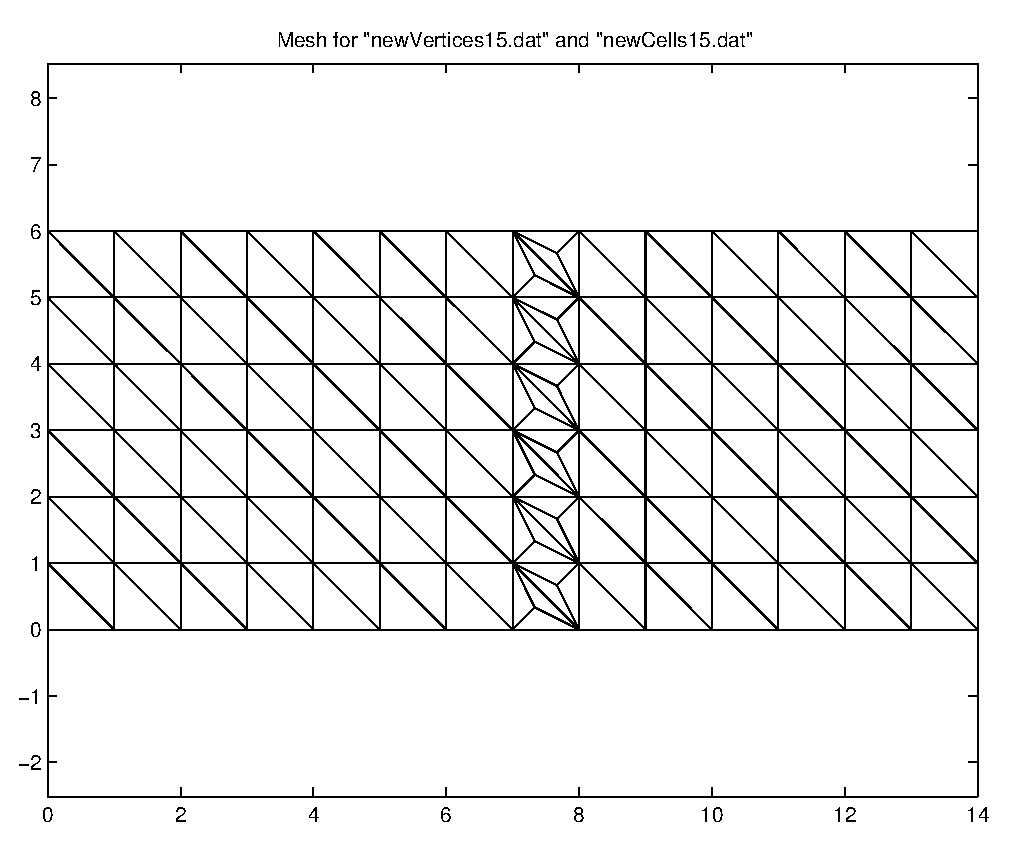
\epsfig{file=output12.eps, width=0.7\textwidth}
\caption{Output 2 of \cref{ATCscs}}
\label{output12}
\end{figure}

\begin{figure}
\centering
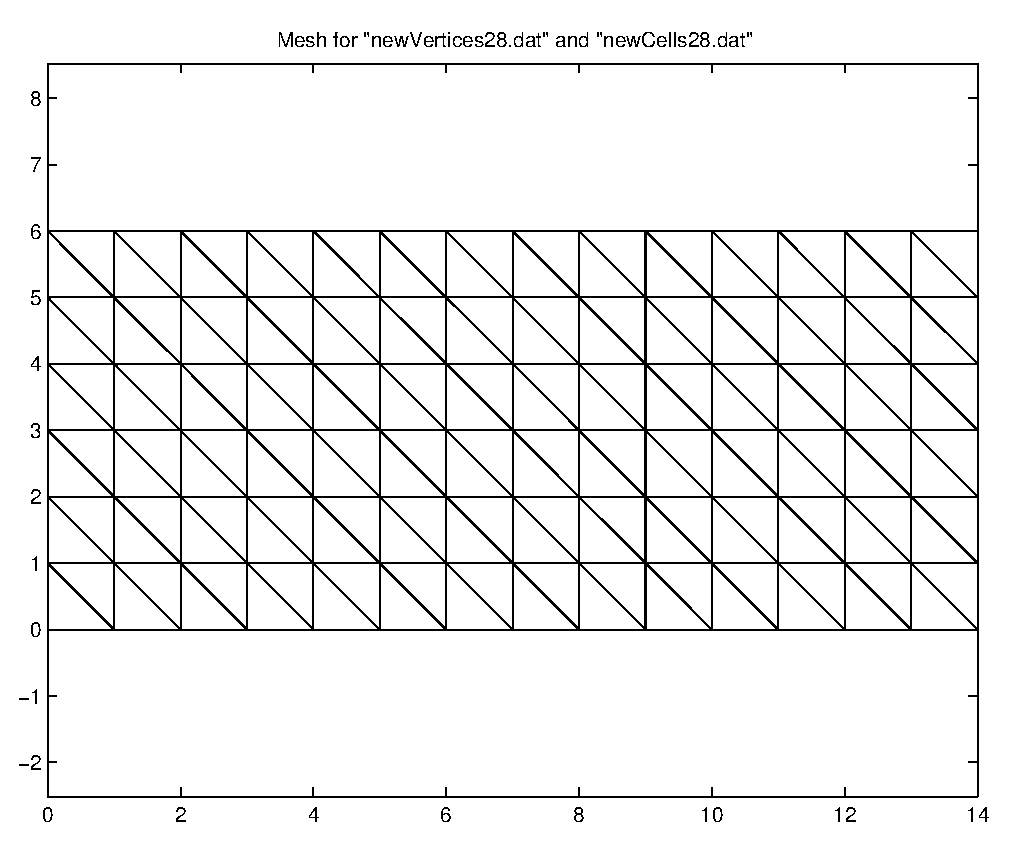
\epsfig{file=output13.eps, width=0.7\textwidth}
\caption{Output 3 of \cref{ATCscs}}
\label{output13}
\end{figure}

\begin{figure}
\centering
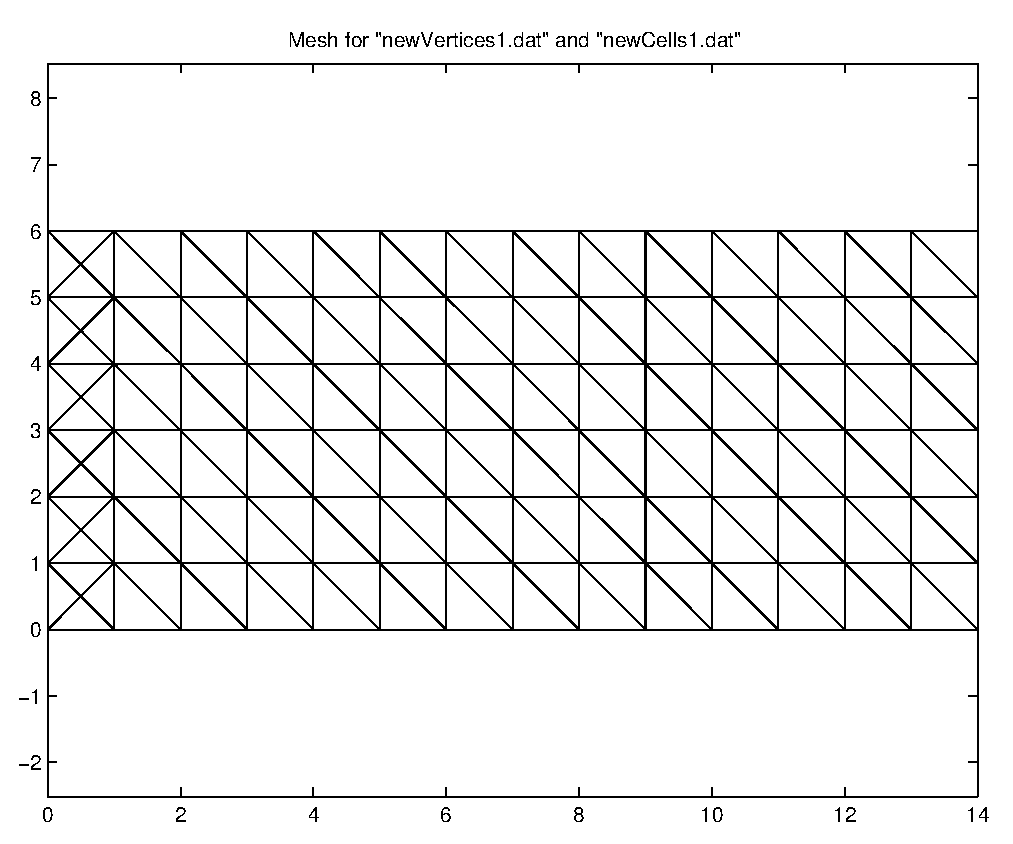
\epsfig{file=output21.eps, width=0.7\textwidth}
\caption{Output 1 of \cref{ATCrcs1}}
\label{output21}
\end{figure}

\begin{figure}
\centering
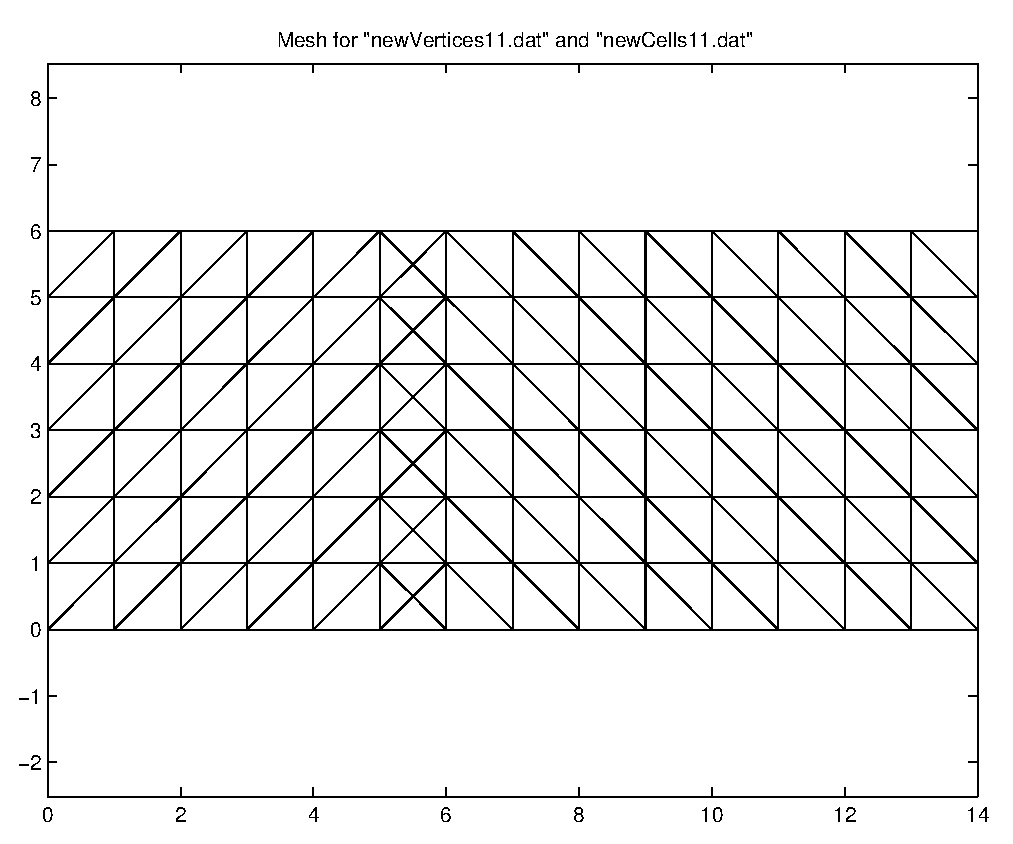
\epsfig{file=output22.eps, width=0.7\textwidth}
\caption{Output 2 of \cref{ATCrcs1}}
\label{output22}
\end{figure}

\begin{figure}
\centering
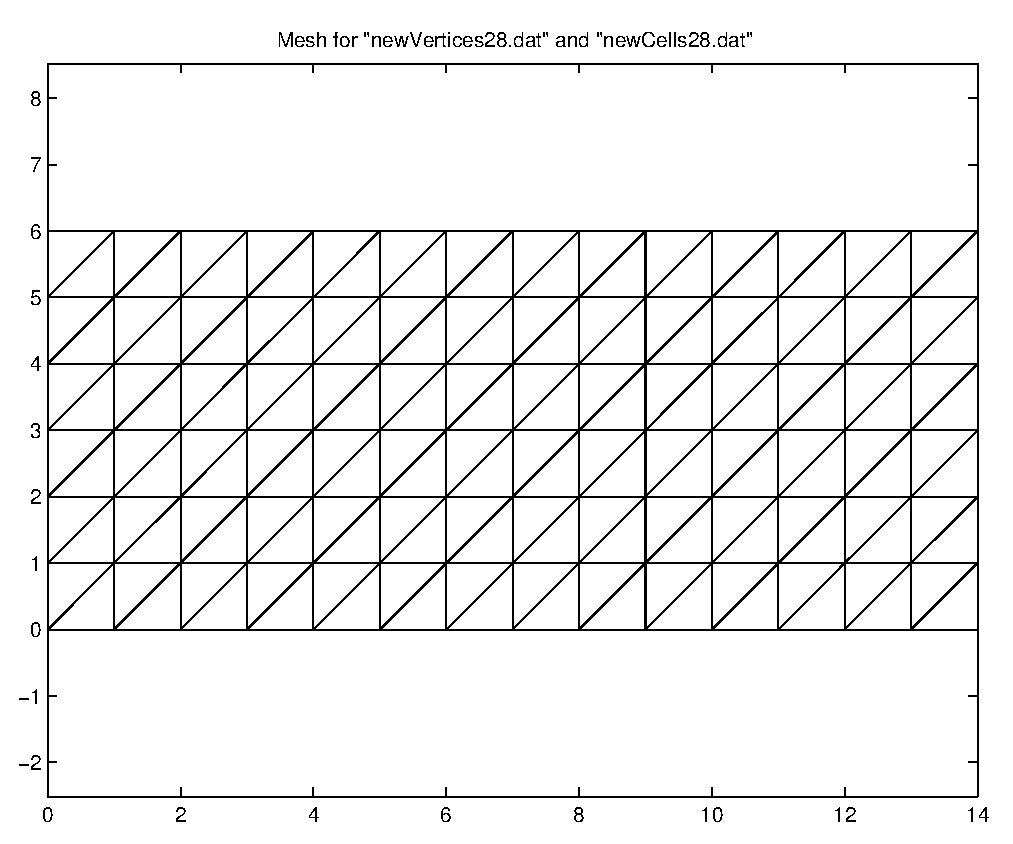
\epsfig{file=output23.eps, width=0.7\textwidth}
\caption{Output 3 of \cref{ATCrcs1}}
\label{output23}
\end{figure}

\clearpage

\begin{figure}
\centering
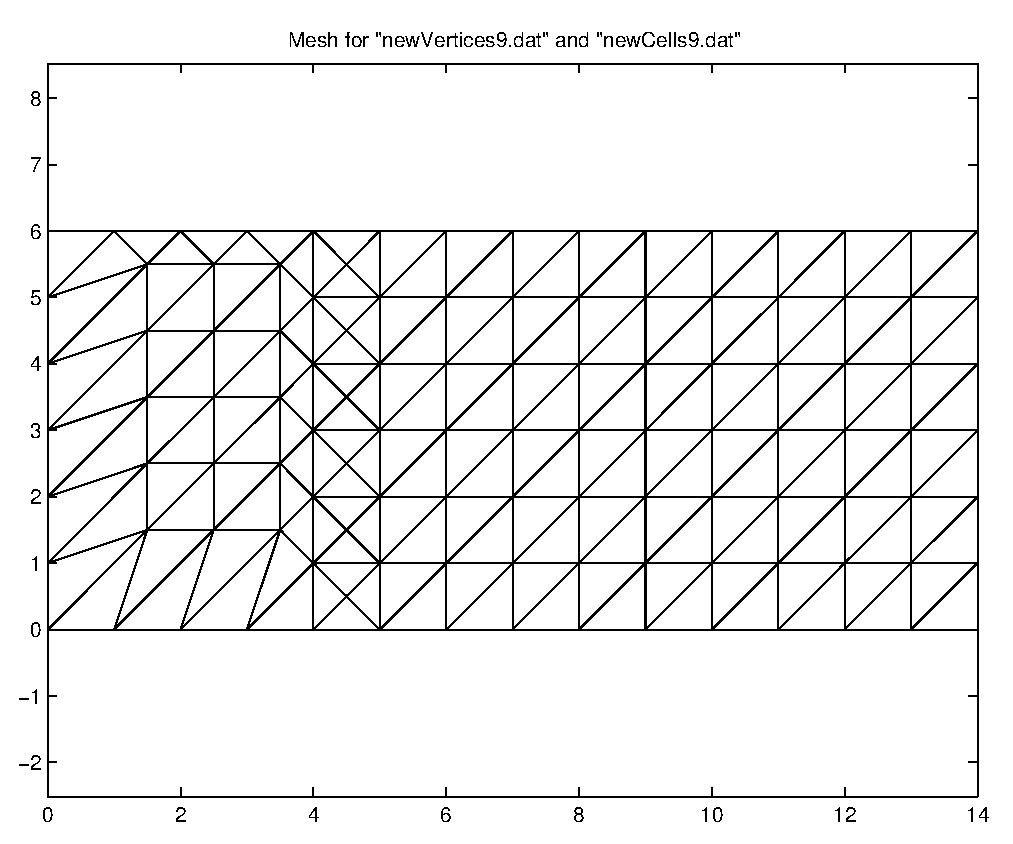
\epsfig{file=output31.eps, width=0.7\textwidth}
\caption{Output 1 of \cref{ATCrcs2}}
\label{output31}
\end{figure}

\begin{figure}
\centering
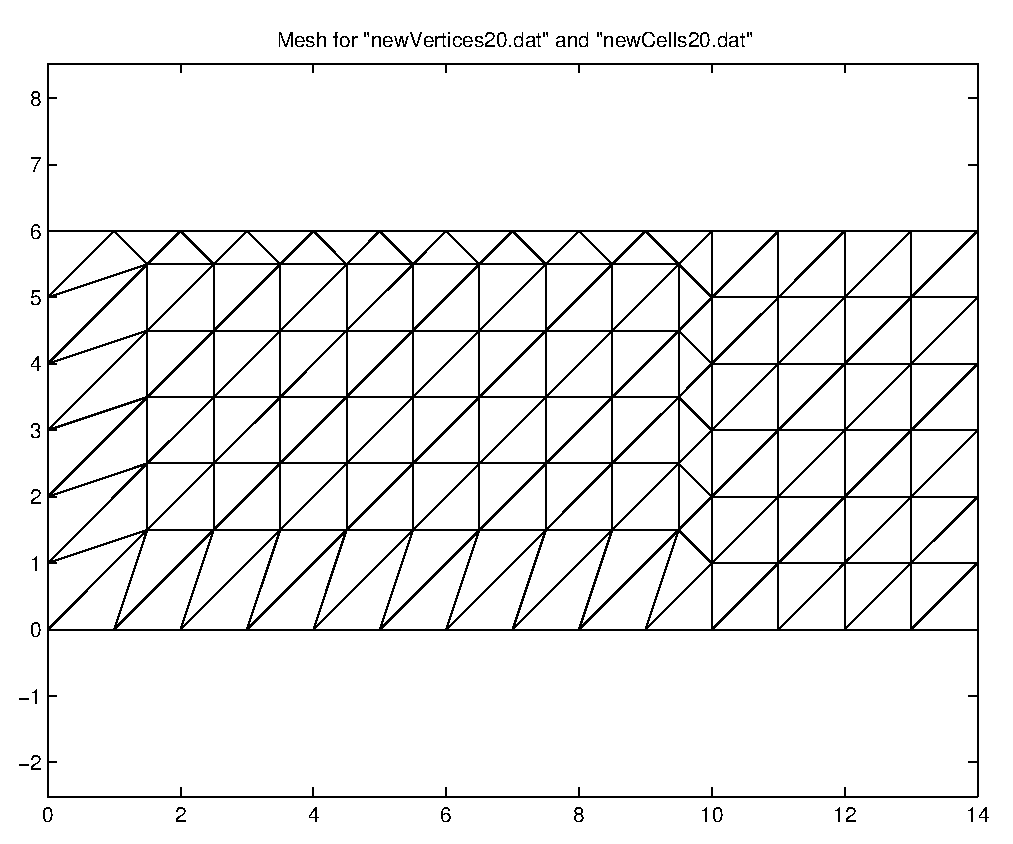
\epsfig{file=output32.eps, width=0.7\textwidth}
\caption{Output 2 of \cref{ATCrcs2}}
\label{output32}
\end{figure}

\begin{figure}
\centering
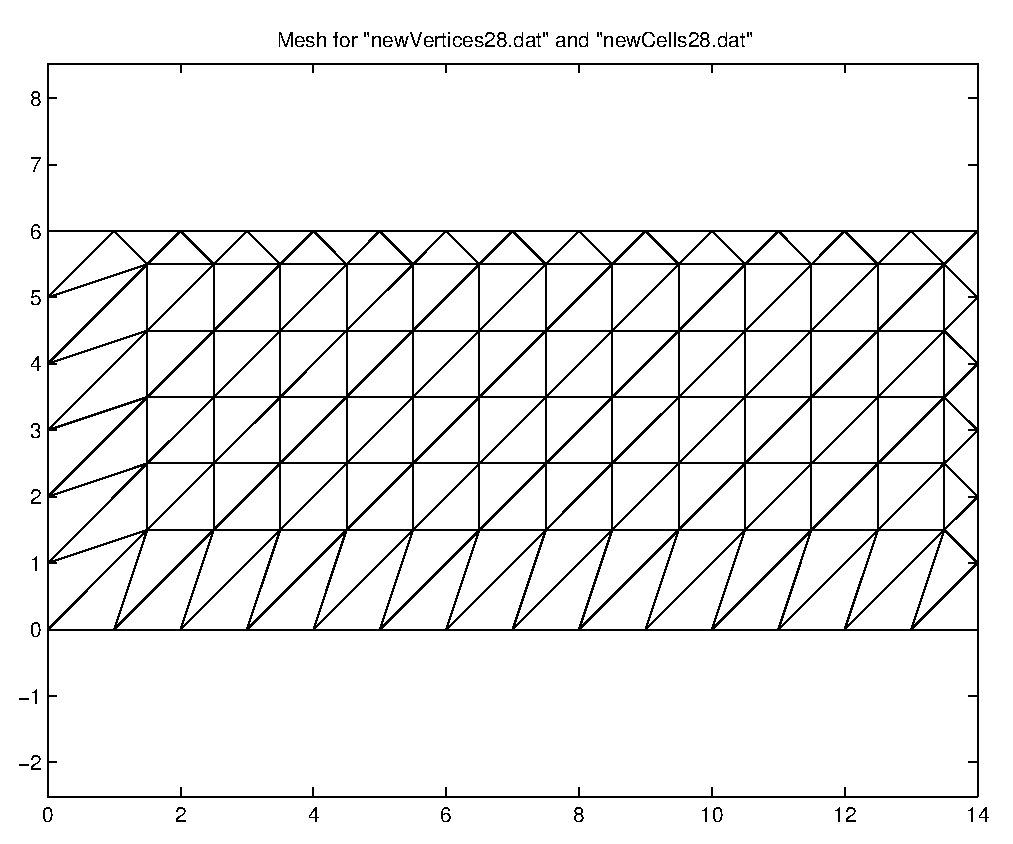
\epsfig{file=output33.eps, width=0.7\textwidth}
\caption{Output 3 of \cref{ATCrcs2}}
\label{output33}
\end{figure}

\begin{figure}
\centering
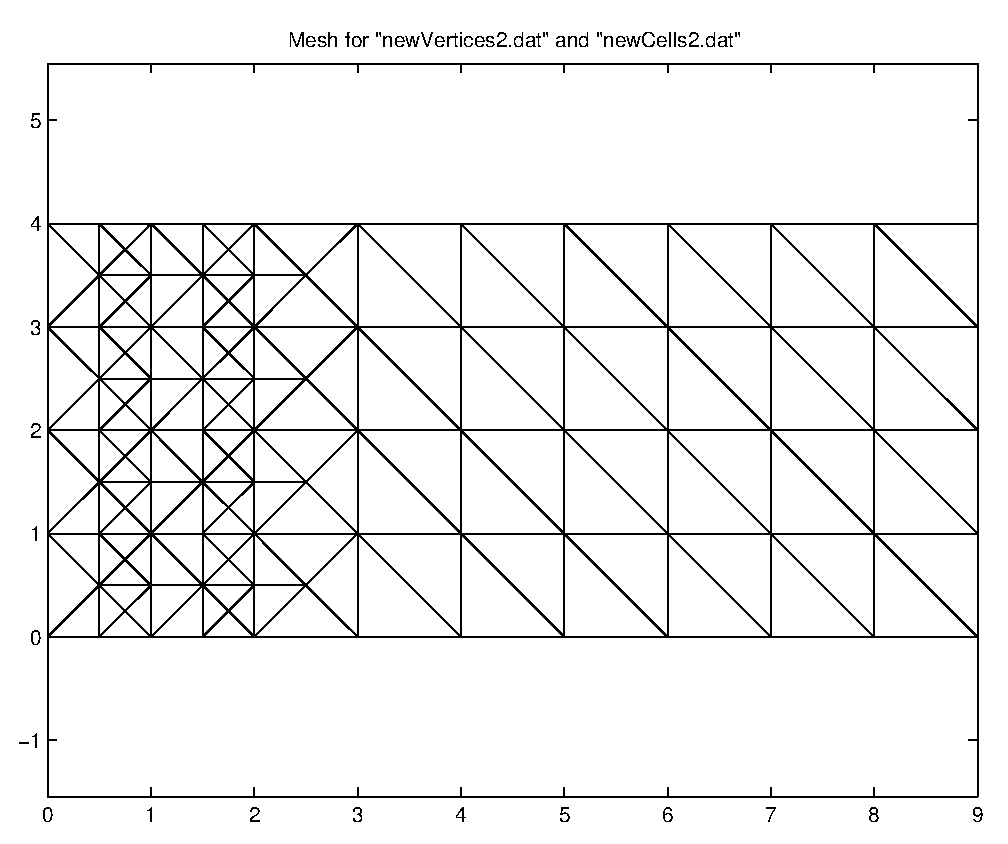
\epsfig{file=output41.eps, width=0.7\textwidth}
\caption{Output 1 of \cref{ATCrcm}}
\label{output41}
\end{figure}

\begin{figure}
\centering
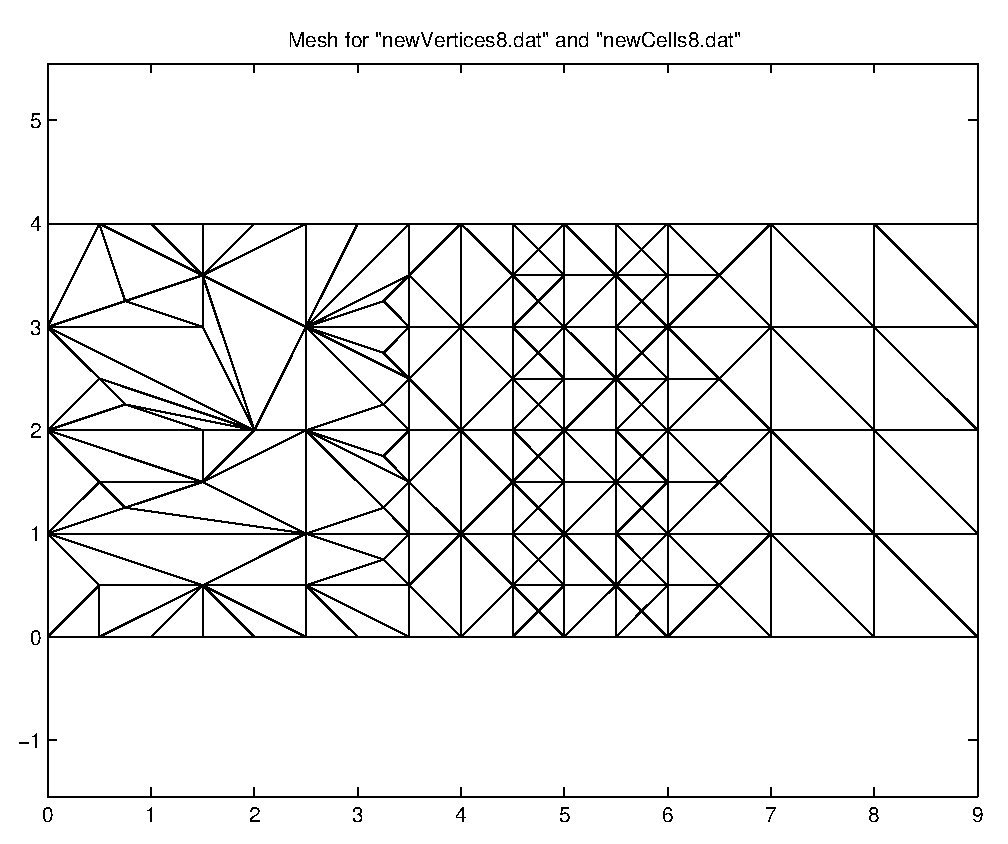
\epsfig{file=output42.eps, width=0.7\textwidth}
\caption{Output 2 of \cref{ATCrcm}}
\label{output42}
\end{figure}

\begin{figure} 
\centering
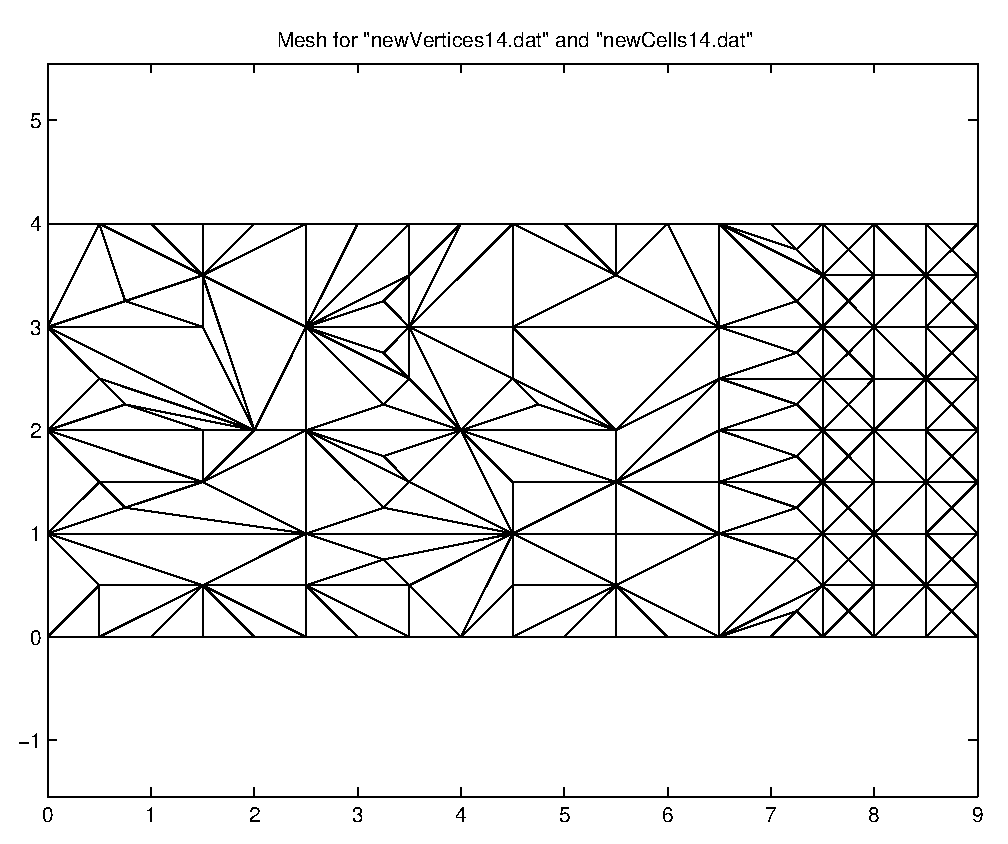
\epsfig{file=output43.eps, width=0.7\textwidth}
\caption{Output 3 of \cref{ATCrcm}}
\label{output43}
\end{figure}

\begin{figure}
\centering
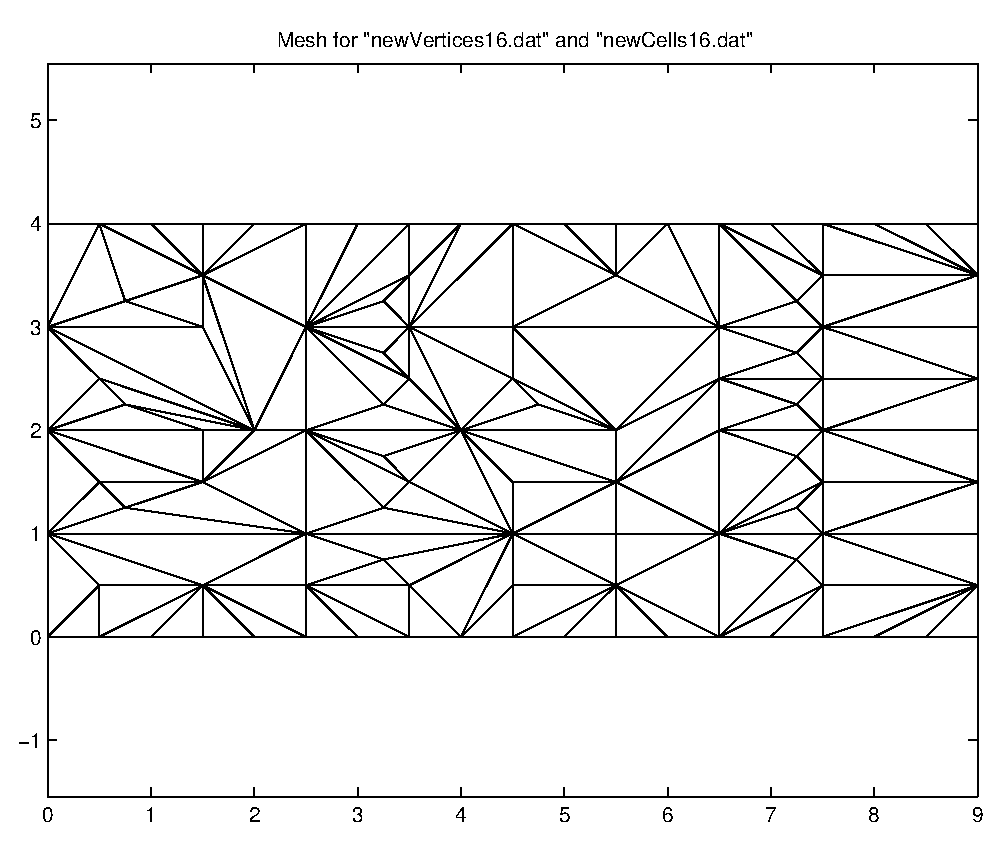
\epsfig{file=output44.eps, width=0.7\textwidth}
\caption{Output 4 of \cref{ATCrcm}}
\label{output44}
\end{figure}


\begin{figure}
\centering
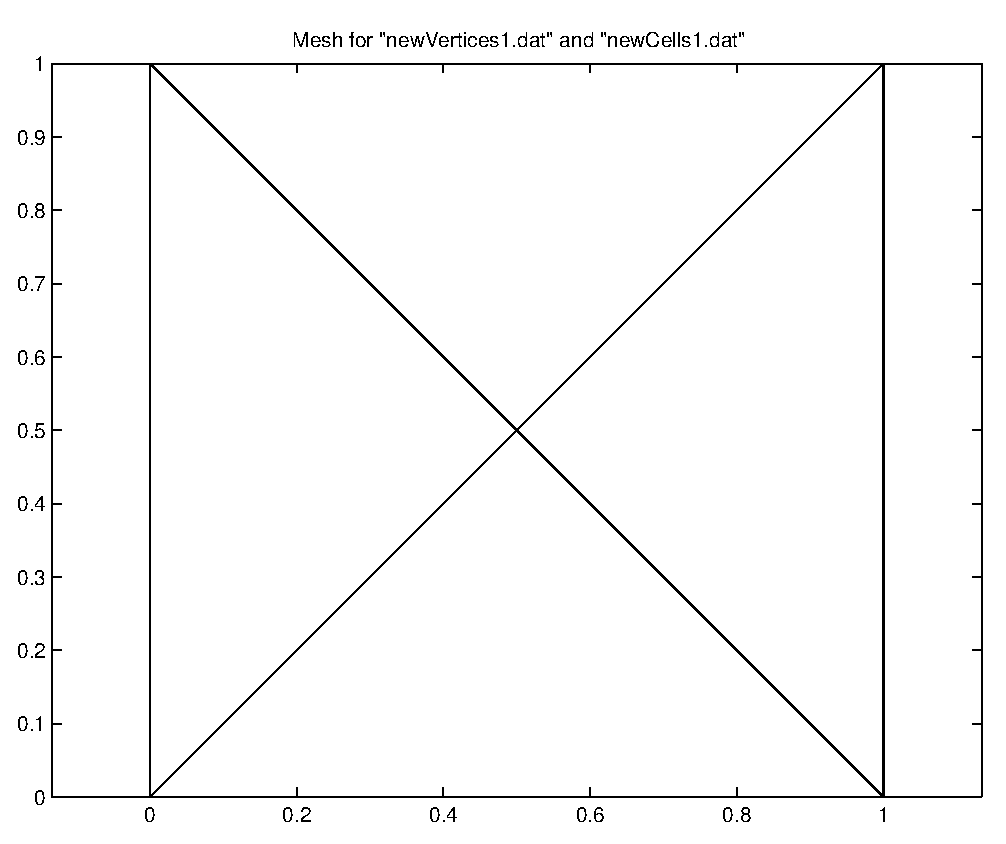
\epsfig{file=output51.eps, width=0.7\textwidth}
\caption{Output 1 of \cref{ATCrm}}
\label{output51}
\end{figure}

\begin{figure}
\centering
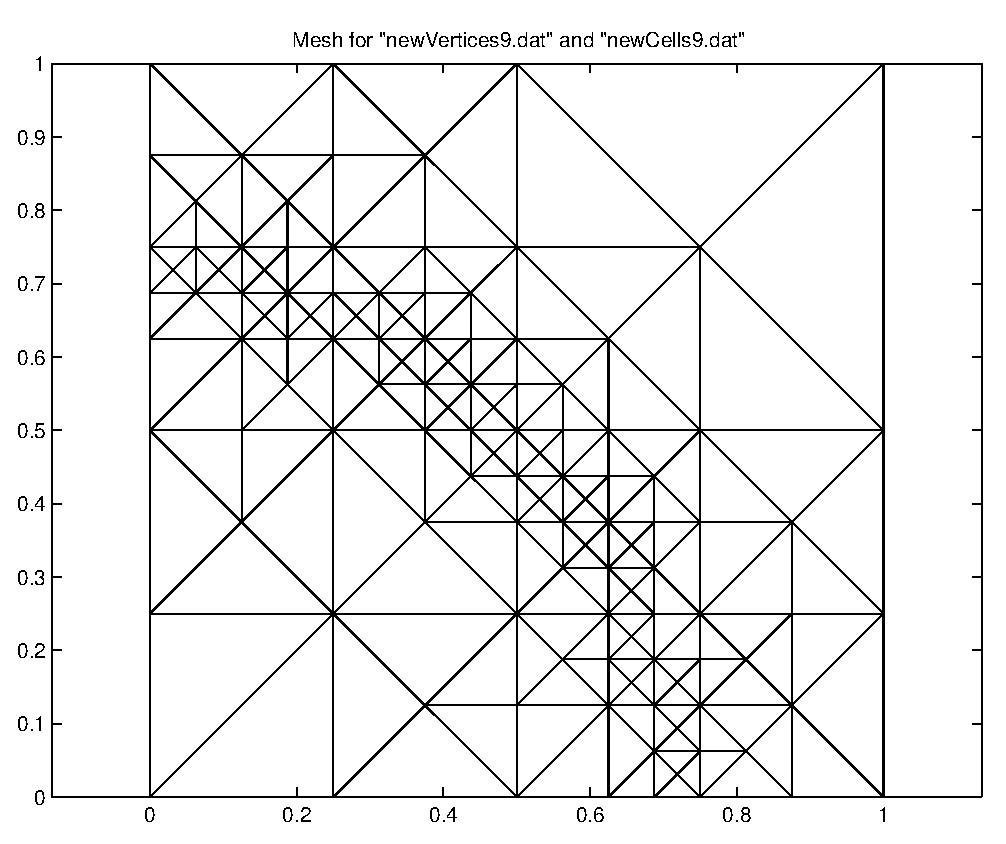
\epsfig{file=output52.eps, width=0.7\textwidth}
\caption{Output 2 of \cref{ATCrm}}
\label{output52}
\end{figure}

\begin{figure}
\centering
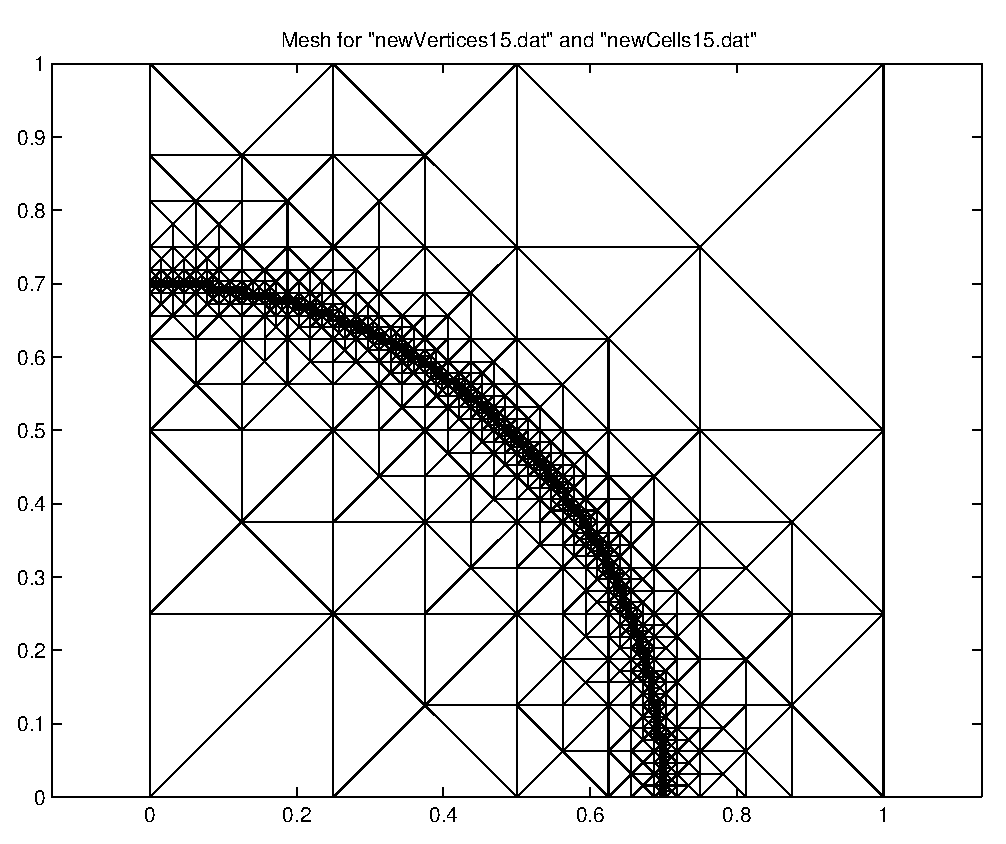
\epsfig{file=output53.eps, width=0.7\textwidth}
\caption{Output 3 of \cref{ATCrm}}
\label{output53}
\end{figure}

%\newpage

%\bibliography{WenRef}
%\bibliographystyle{plainnat}

\end{document}
